

\documentclass[10pt,twocolumn,letterpaper]{article}

%%%%%%%%% PAPER TYPE  - PLEASE UPDATE FOR FINAL VERSION
% \usepackage[review]{cvpr}      % To produce the REVIEW version
\usepackage{cvpr}              % To produce the CAMERA-READY version
%\usepackage[pagenumbers]{cvpr} % To force page numbers, e.g. for an arXiv version

% Include other packages here, before hyperref.
\usepackage{graphicx}
\usepackage{amsmath}
\usepackage{amssymb}
\usepackage{booktabs}
\usepackage[shortlabels]{enumitem}
\usepackage{float}



% It is strongly recommended to use hyperref, especially for the review version.
% hyperref with option pagebackref eases the reviewers' job.
% Please disable hyperref *only* if you encounter grave issues, e.g. with the
% file validation for the camera-ready version.
%
% If you comment hyperref and then uncomment it, you should delete
% ReviewTempalte.aux before re-running LaTeX.
% (Or just hit 'q' on the first LaTeX run, let it finish, and you
%  should be clear).
\usepackage[pagebackref,breaklinks,colorlinks]{hyperref}


% Support for easy cross-referencing
\usepackage[capitalize]{cleveref}
\crefname{section}{Sec.}{Secs.}
\Crefname{section}{Section}{Sections}
\Crefname{table}{Table}{Tables}
\crefname{table}{Tab.}{Tabs.}


%%%%%%%%% PAPER ID  - PLEASE UPDATE
\def\cvprPaperID{*****} % *** Enter the CVPR Paper ID here
\def\confName{CVPR}
\def\confYear{2023}


\begin{document}

%%%%%%%%% TITLE - PLEASE UPDATE
\title{NTIRE 2023 Efficient SR Challenge Factsheet\\-Efficient Feature Distillation Network-}
\author{Mingjian Zhang , Jingpeng Shi\\
Anhui University, Hefei, China\\
{\tt\small hukangyy@gmail.com},{\tt\small jinpeeeng.s@gmail.com}
% For a paper whose authors are all at the same institution,
% omit the following lines up until the closing ``}''.
% Additional authors and addresses can be added with ``\and'',
% just like the second author.
% To save space, use either the email address or home page, not both
}
\maketitle

\newcommand{\github}[1]{\href{https://github.com/#1/}{github.com/#1}}


\section{Team Details}

\begin{itemize}
	\item Team name: \textbf{FRL Team 05}                                  
	\item Team leader name: \textbf{Mingjian Zhang }                          
	\item Team leader address, phone number, and email:
	\begin{itemize}
		\item address: \textbf{Anhui University, Hefei, China}
		\item phone number: \textbf{+86 136 6742 1529}
		\item email: \textbf{zhang9317112@gmail.com}
	\end{itemize}
	\item Rest of the team members: \textbf{Jinpeng Shi (advisor)}        
	\item Team website URL (if any): \\ \github{Fried-Rice-Lab/FriedRiceLab}                   
	\item Affiliation: \textbf{Anhui University}
	\item Affiliation of the team and/or team members with NTIRE 2023 sponsors (check the workshop website): \textbf{N/A}
	\item User names and entries on the NTIRE 2023 Codalab competitions (development/validation and testing phases):
	\begin{itemize}
		\item user name: \textbf{zhang9317112}
		\item development entries: \textbf{2}
		\item validation entries: \textbf{17}
	\end{itemize}
	\item Best scoring entries of the team during development/validation phase:
	\begin{table}[h]
		\centering
		\resizebox{\linewidth}{!}{
			\begin{tabular}{|c|c|c|c|c|}
				\hline
				PSNR&SSIM&Runtime&Params&Extra Data\\\hline
				29.02  (10) &0.83 (9)& 0.09 (28)& 244558.00 (21) &1.00 (1)\\
				\hline
			\end{tabular}
		}
	\end{table}
	\item Link to the codes/executables of the solution(s): \\ \github{zhang9317112/NTIRE2023\_ESR}
\end{itemize}

\textbf{Fried Rice Lab} (FRL) is organized by students from Anhui University who are interested in image restoration. FRL is dedicated to proposing clean and efficient image restoration solutions and contributing to the image restoration open source community. \textbf{FRL Team 05}, led by Mingjian Zhang and advised by Jinpeng Shi, was among the teams that FRL sent to compete in the NTIRE 2023 ESR competition, with \textit{Someone (replace if any)} completing the roster.

\section{Method Details}

The structure is inspired by classical SR structure——CNN(Convolutional Neural Network) and Transformer structure which is a common-used in SR area.
Nowadays, transformer is widely used in lightweight sr tasks. However, we know from ConvneXt\cite{ref1} that CNN is not inferior to trans in performance in many cases. from this idea we analyze the advantages of each of Transformer(Likes Swin transformer\cite{ref2}) and CNN, and propose RB(Residual Block) based on the most classic SR network EDSR\cite{ref3} with changes, adding a DSB(Dimensional Separable Block) which is similar to the transformer' self-attention mechanism to obtain long-range connections.We also add a nonlinear activation function to stabilize the training.

As shown in Fig1, our structure have three modules:(1)3*3 kernel convolution(shallow feature extraction).(2)Basic Layer(deep feature extraction).(3)3*3 kernel convolution and sub-Pixel(HR-image reconstruction).Our main contribution is to creatively present a useful layer called Basic Layer,which can process information efficiently.

\subsection{Block Layer}
Block Layer is the main layer in this structure.This Layer includes the following two modules——Dimensional separable Block and Residual Block.

\subsection{Residual Block}
Residual Block is improved by the classical convolutional stacking module of EDSR, which removes the BatchNorm and considers it redundant. But we found that LayerNorm\cite{ref4} is suitable with SR tasks, so we added LayerNorm to that module to improve the performance.

\subsection{Dimensional Separable Block}
Poolformer\cite{ref5} confirmed that th advantage of transformer is its backbone structure and its self-attention can be replaced by convolution.
Inspiring by Depthwise Separable Convolution\cite{ref6},We propose Dimensional Separable Block to divide the information features into H(Height), W(Weight), and C(Channel). 
From Mobilenets,\cite{ref7} the feature information is divided into PW(PointWise) and DW(DepthWise), and we process the H and W information together for PW (intra-channel feature information) and then use c for DW (inter-channel feature information). From Simple baselines for image restoration\cite{ref8}, we know that the information of H and W is multiplied in front to achieve his nonlinearity, then finally outputs features. From Inception-ResNet\cite{ref9}, we know that the convolution kernel is decomposed so as to maintain performance while greatly reducing the parameters,So we use grouped convolution for feature extraction of H and W.




\begin{figure}
	\centering
	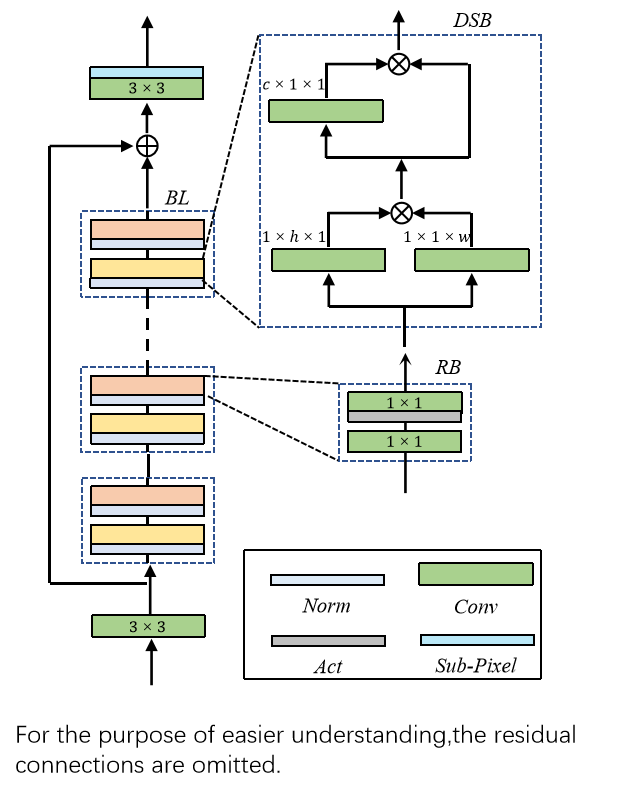
\includegraphics[width=1.0\linewidth]{../competition_picture1}
	\caption{The architecture of Super Resolution Net-X (SRneXt)}
	\label{fig:competitionpicture1}
\end{figure}



 



\subsection{Training Details}
Training was performed on DIV2K \cite{ref10} and Flickr2K \cite{ref11} images. HR patches of size 256 × 256 were randomly cropped from the HR images and the mini-batch size was set to 128. The model was trained with the ADAM optimizer\cite{ref12}, where $\beta_1 =0.9$ and $\beta_2 =0.9999$. The initial learning rate was set to 5 × $10^{-4}$ with cosine learning rate decay. The L2 loss was used for ab initio training and the number of iterations The model was implemented using Pytorch 1.10.1 and trained on 2 GeForce RTX 3090 GPUs.


\subsection{Experimental Results}
The experimental result is shown in Tbale \ref{tab:result}. FLOPs and Activation are tested on an LR image of size $256\times 256$. PNSR[val] is tested on DIV2k validation dataset, while PSNR[test] is calculated on a combination of DIV2K and LSDIR test data. The runtime is is evaluated on DIV2K and LSDIR test datasets using a single GeForce RTX 3090 GPU. 

 \begin{table}[t]
	\centering
	\begin{tabular}{|c|c|c|c|}\hline
		PSNR[val]&PSNR[test]& Params[M]& FLOPs[G] \\
		\hline
		
		29.02&27.02&  0.2445&15.376\\
		\hline
		 GPU Mem.[M] & Activation[M]&Average Runtime[ms]&Conv2d \\
		\hline
		
		448.6826&422.903&91.16&158\\
		\hline
	\end{tabular}
	\caption{Result for NTIRE2023 ESR Challenge. FLOPs and Activation are tested on an LR image of size $256\times 256$. The runtime is is averaged on DIV2K and LSDIR test datasets using a single NVIDIA RTX 3090 GPU.}
	\label{tab:result}
 \end{table}



\section{Other details}
\begin{itemize}
\item Planned submission of a solution(s) description paper at NTIRE 2023 workshop.

We are not planning to submit the solution description paper to NTIRE2023 workshop, since it has been submitted to other conference.

\item General comments and impressions of the NTIRE 2023 challenge. 

The organizers provided detailed processes and instructions and we appreciate the effort they spent!

\end{itemize}

%%%%%%%%% REFERENCES
{\small
\begin{thebibliography}{100} 
	
	\bibitem{ref1} Liu Z, Mao H, Wu C Y, et al. A convnet for the 2020s[C]//Proceedings of the IEEE/CVF Conference on Computer Vision and Pattern Recognition. 2022: 11976-11986.
	
	\bibitem{ref2}Liu Z, Lin Y, Cao Y, et al. Swin transformer: Hierarchical vision transformer using shifted windows[C]//Proceedings of the IEEE/CVF international conference on computer vision. 2021: 10012-10022.
	
	\bibitem{ref3} Lim B, Son S, Kim H, et al. Enhanced deep residual networks for single image super-resolution[C]//Proceedings of the IEEE conference on computer vision and pattern recognition workshops. 2017: 136-144.
 
    \bibitem{ref4}Ba J L, Kiros J R, Hinton G E. Layer normalization[J]. arXiv preprint arXiv:1607.06450, 2016.

    \bibitem{ref5}Yu W, Luo M, Zhou P, et al. Metaformer is actually what you need for vision[C]//Proceedings of the IEEE/CVF conference on computer vision and pattern recognition. 2022: 10819-10829.

    \bibitem{ref6}Chollet F. Xception: Deep learning with depthwise separable convolutions[C]//Proceedings of the IEEE conference on computer vision and pattern recognition. 2017: 1251-1258.
    
     \bibitem{ref7}Howard A G, Zhu M, Chen B, et al. Mobilenets: Efficient convolutional neural networks for mobile vision applications[J]. arXiv preprint arXiv:1704.04861, 2017.
    
     \bibitem{ref8}Chen L, Chu X, Zhang X, et al. Simple baselines for image restoration[C]//Computer Vision–ECCV 2022: 17th European Conference, Tel Aviv, Israel, October 23–27, 2022, Proceedings, Part VII. Cham: Springer Nature Switzerland, 2022: 17-33.
     
     \bibitem{ref9}Szegedy C, Ioffe S, Vanhoucke V, et al. Inception-v4, inception-resnet and the impact of residual connections on learning[C]//Proceedings of the AAAI conference on artificial intelligence. 2017, 31(1).
     
     \bibitem{ref10}Eirikur Agustsson and Radu Timofte. Ntire 2017 challenge on single image super-resolution: Dataset and study. In CVPR workshops, pages 126–135, 2017.
     
     \bibitem{ref11}Radu Timofte, Eirikur Agustsson, Luc Van Gool, Ming Hsuan Yang, and Lei Zhang. Ntire 2017 challenge on single image super-resolution: Methods and results. In CVPR workshops, pages 114–125, 2017.
	
	
	
\end{thebibliography}
}

\end{document}
